%%%%%%%%%%%%%%%%%%%%%%%%%%%%%%%%%%%%%%%%%
% baposter Landscape Poster
% LaTeX Template
% Version 1.0 (11/06/13)
%
% baposter Class Created by:
% Brian Amberg (baposter@brian-amberg.de)
%
% This template has been downloaded from:
% http://www.LaTeXTemplates.com
%
% License:
% CC BY-NC-SA 3.0 (http://creativecommons.org/licenses/by-nc-sa/3.0/)
%
%%%%%%%%%%%%%%%%%%%%%%%%%%%%%%%%%%%%%%%%%

%----------------------------------------------------------------------------------------
%	PACKAGES AND OTHER DOCUMENT CONFIGURATIONS
%----------------------------------------------------------------------------------------

\documentclass[landscape,a0paper,fontscale=0.285]{baposter} % Adjust the font scale/size here

\usepackage{graphicx} % Required for including images
\graphicspath{{figures/}} % Directory in which figures are stored

\usepackage[utf8]{inputenc}
\usepackage[german]{babel}
\usepackage[T1]{fontenc}

\usepackage{amsmath} % For typesetting math
\usepackage{amssymb} % Adds new symbols to be used in math mode

\usepackage{booktabs} % Top and bottom rules for tables
\usepackage{enumitem} % Used to reduce itemize/enumerate spacing
\usepackage{palatino} % Use the Palatino font
\usepackage[font=small,labelfont=bf]{caption} % Required for specifying captions to tables and figures

\usepackage{multicol} % Required for multiple columns
\setlength{\columnsep}{1.5em} % Slightly increase the space between columns
\setlength{\columnseprule}{0mm} % No horizontal rule between columns

\usepackage{chemmacros}

\usepackage{tikz} % Required for flow chart
\usetikzlibrary{shapes,arrows} % Tikz libraries required for the flow chart in the template

\newcommand{\compresslist}{ % Define a command to reduce spacing within itemize/enumerate environments, this is used right after \begin{itemize} or \begin{enumerate}
\setlength{\itemsep}{1pt}
\setlength{\parskip}{0pt}
\setlength{\parsep}{0pt}
}

\definecolor{lightblue}{rgb}{0.145,0.6666,1} % Defines the color used for content box headers

\begin{document}

\begin{poster}
{
headerborder=closed, % Adds a border around the header of content boxes
colspacing=1em, % Column spacing
bgColorOne=white, % Background color for the gradient on the left side of the poster
bgColorTwo=white, % Background color for the gradient on the right side of the poster
borderColor=lightblue, % Border color
headerColorOne=black, % Background color for the header in the content boxes (left side)
headerColorTwo=lightblue, % Background color for the header in the content boxes (right side)
headerFontColor=white, % Text color for the header text in the content boxes
boxColorOne=white, % Background color of the content boxes
textborder=roundedleft, % Format of the border around content boxes, can be: none, bars, coils, triangles, rectangle, rounded, roundedsmall, roundedright or faded
eyecatcher=true, % Set to false for ignoring the left logo in the title and move the title left
headerheight=0.1\textheight, % Height of the header
headershape=roundedright, % Specify the rounded corner in the content box headers, can be: rectangle, small-rounded, roundedright, roundedleft or rounded
headerfont=\Large\bf\textsc, % Large, bold and sans serif font in the headers of content boxes
%textfont={\setlength{\parindent}{1.5em}}, % Uncomment for paragraph indentation
linewidth=2pt % Width of the border lines around content boxes
}
%----------------------------------------------------------------------------------------
%	TITLE SECTION 
%----------------------------------------------------------------------------------------
%
{
\includegraphics[height=4em, width=20em]{logo.png}} % First university/lab logo on the left
{\bf\textsc{Direkte Analyse von Chlorophyllkataboliten}\vspace{0.5em}} % Poster title
{\textsc{\ Florian Kluibenschedl \ \hspace{12pt} 8a, BRG Telfs - 2017/18}} % Author names and institution
%{
\includegraphics[height=4em, width=18em]{logo.png}} % Second university/lab logo on the right

%----------------------------------------------------------------------------------------
%	OBJECTIVES
%----------------------------------------------------------------------------------------

\headerbox{Objectives}{name=objectives,column=0,row=0}{

Das Ziel bestand darin, die Abbauprodukte des Chlorophylls einer direkten massenspektrometrischen Analyse zu unterziehen. Im Rahmen dessen wurden diverse Meilensteine gesetzt: 

\begin{enumerate}\compresslist
\item MS-Leafspray als Analysemethode
\item Identifikation von Chl-Kataboliten
\item Synthese eines Anhydrids
\item Erstellen von Fragmentierungsdiagrammen
\item Verbesserung der Möglichkeiten der Strukturaufklärung
\end{enumerate}

\vspace{0.3em} % When there are two boxes, some whitespace may need to be added if the one on the right has more content
}

%----------------------------------------------------------------------------------------
%	INTRODUCTION
%----------------------------------------------------------------------------------------

\headerbox{Introduction}{name=introduction,column=1,row=0,bottomaligned=objectives}{

Die alljährliche Laubfärbung ist eines der sichtbarsten Zeichen von Leben und damit auch aus dem All beobachtbar. Bei diesem Prozess wird der grüne Blattfarbstoff (= Chlorophyll) abgebaut. In der vorliegenden Arbeit galt es, diese Abbauprodukte mithilfe eines Massenspektrometers zu untersuchen. 

Dabei wurde besonderes Augenmerk auf die Verbesserung massenspektrometrischer Methoden gelegt,  indem das Verhalten von Chl-Kataboliten des Brokkoliblattes im Massenspektrometer genauer untersucht wurde. 
}

%----------------------------------------------------------------------------------------
%	RESULTS 2
%----------------------------------------------------------------------------------------

\headerbox{Results II - Fragmentierungsdiagramme}{name=results,column=2,span=2,row=0}{

\begin{multicols}{2}
\vspace{1em}
\begin{center}
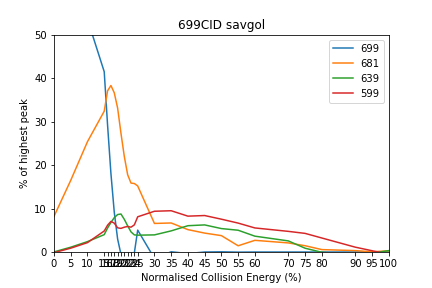
\includegraphics[width=0.4\textwidth]{699CID-savgol1}
\captionof{figure}{Fragmentierungsdiagramm Reaktionsprodukt des \textit{Bo}-DNCC, m/z = 699 [M+H]\textsuperscript{+}}
\end{center}

Im Rahmen der massenspektrometrischen Untersuchungen wurden Fragmentierungsdiagramme der Chl-Kataboliten und deren Reaktionsprodukte erstellt. Dabei wurden die Verbindungen im Massenspektrometer mit unterschiedlichen Energien angeregt und die Intensitäten der auftretenden Fragmentierungen (=Abspaltungen) gemessen. \\

In Abbildung 1 ist das Fragmentierungsdiagramm des Reaktionsproduktes des \textit{Bo}-DNCC dargestellt. Auf der Ordinate wird dabei die Anregungsenergie und auf der Abszisse die Intensitäten der Fragmente aufgetragen. 
\end{multicols}

%------------------------------------------------

\begin{multicols}{2}
\vspace{1em}
In Abbildung 2 wird ein Strukturvorschlag für das Reaktionsprodukt des \textit{Bo}-DNCC gemacht. Zu beachten ist das Anhydrid, das über eine Abspaltung von 60 Da identifiziert werden konnte. Ein Mechanismus für diese Abspaltung wird ebenfalls vorgeschlagen, indem durch Pfeile die Bewegung der Elektronen gekennzeichnet wird.  

\begin{center}
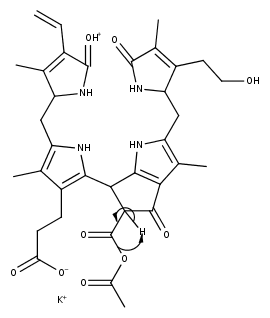
\includegraphics[width=0.8\linewidth, height=0.3\textheight]{VWA_Katabolit_699-639_MK_electronMovement}
\captionof{figure}{Figure caption}
\end{center}

\end{multicols}
}

%----------------------------------------------------------------------------------------
%	REFERENCES
%----------------------------------------------------------------------------------------

\headerbox{References}{name=references,column=0,above=bottom}{

\renewcommand{\section}[2]{\vskip 0.05em} % Get rid of the default "References" section title
\nocite{*} % Insert publications even if they are not cited in the poster
\small{ % Reduce the font size in this block
\bibliographystyle{unsrt}
\bibliography{sample} % Use sample.bib as the bibliography file
}}

%----------------------------------------------------------------------------------------
%	FUTURE RESEARCH
%----------------------------------------------------------------------------------------

\headerbox{Future Research}{name=futureresearch,column=1,span=2,aligned=references,above=bottom}{ % This block is as tall as the references block

\begin{multicols}{2}
Die vorliegende Arbeit beschäftigt sich mit Grundlagenforschung im Bereich der Strukturaufklärung. Besonders die Verfolgung der Idee der Fragmentierungsdiagramme eignet sich für weitere Forschungen, wobei diese noch verifiziert werden müssten. Auch MS-Leafspray eignet sich für die Weiterentwicklung schneller und effizienter Analysen.
\end{multicols}
}

%----------------------------------------------------------------------------------------
%	CONTACT INFORMATION
%----------------------------------------------------------------------------------------

\headerbox{Contact Information}{name=contact,column=3,aligned=references,above=bottom}{ % This block is as tall as the references block

\begin{description}\compresslist
\item[Web] github.com/Progklui/vwaFloKlui/
\item[Email] florian.kluibenschedl@live.de
\item[Phone] +43 699 16056980
\end{description}
}

%----------------------------------------------------------------------------------------
%	CONCLUSION
%----------------------------------------------------------------------------------------

\headerbox{Conclusion}{name=conclusion,column=2,span=2,row=0,below=results,above=references}{

\begin{multicols}{2}

%\tikzstyle{decision} = [diamond, draw, fill=blue!20, text width=4.5em, text badly centered, node distance=2cm, inner sep=0pt]
%%\tikzstyle{block} = [rectangle, draw, fill=blue!20, text width=5em, text centered, rounded corners, minimum height=4em]
%\tikzstyle{line} = [draw, -latex']
%\tikzstyle{cloud} = [draw, ellipse, fill=red!20, node distance=3cm, minimum height=2em]

%\begin{tikzpicture}[node distance = 2cm, auto]
%\node [block] (init) {Initialize Model};
%\node [cloud, left of=init] (Start) {Start};
%\node [cloud, right of=init] (Start2) {Start Two};
%\node [block, below of=init] (init2) {Initialize Two};
%\node [decision, below of=init2] (End) {End};
%\path [line] (init) -- (init2);
%\path [line] (init2) -- (End);
%\path [line, dashed] (Start) -- (init);
%\path [line, dashed] (Start2) -- (init);
%\path [line, dashed] (Start2) |- (init2);
%\end{tikzpicture}

%------------------------------------------------

Im Rahmen der experimentellen Untersuchungen konnte der Großteil der Forschungsfragen behandelt werden. Mit MS-Leafspray wurde eine moderne Analysemethode verwendet, die eine schnelle Identifikation der Chl-Kataboliten erlaubte. Forschungspotential noch vorhanden!
%\begin{itemize}\compresslist
%\item Pellentesque eget orci eros. Fusce ultricies, tellus et pellentesque fringilla, ante massa luctus libero, quis tristique purus urna nec nibh. Phasellus fermentum rutrum elementum. Nam quis justo lectus.
%\item Vestibulum sem ante, hendrerit a gravida ac, blandit quis magna.
%\item Donec sem metus, facilisis at condimentum eget, vehicula ut massa. Morbi consequat, diam sed convallis tincidunt, arcu nunc.
%\item Nunc at convallis urna. isus ante. Pellentesque condimentum dui. Etiam sagittis purus non tellus tempor volutpat. Donec et dui non massa tristique adipiscing.
%\end{itemize}

\end{multicols}
}

%----------------------------------------------------------------------------------------
%	MATERIALS AND METHODS
%----------------------------------------------------------------------------------------

\headerbox{Materials \& Methods}{name=method,column=0,below=objectives,bottomaligned=conclusion}{ % This block's bottom aligns with the bottom of the conclusion block

Folgende Geräte wurden für die spektroskopischen und spektrometrischen Untersuchungen verwendet:

\begin{itemize}\compresslist
\item Thermo LCQ DecaXP
\item Thermo LTQ Orbitrap XL
\item Shimadzu HPLC system
\item Online UV/Vis Detektor
\end{itemize}

Das Probenmaterial wurde täglich im Garten meiner Oma gesammelt. Es handelte sich hierbei um bereits seneszente Brokkoliblätter. \\

Die Analyse mit MS-Leafspray erforderte die Entwicklung einer besonderen Blatt-Vorbereitungsmethode:

\begin{itemize}\compresslist
\item zuschneiden des Blattes und Filterpapier
\item herstellen eines Päckchens 
\item einrichten des Päckchens vor dem Massenspektrometer
\item optimieren des Signals
\item Messen und Analyse
\end{itemize}

}

%----------------------------------------------------------------------------------------
%	RESULTS 2
%----------------------------------------------------------------------------------------

\headerbox{Results I}{name=results2,column=1,below=objectives,bottomaligned=conclusion}{ % This block's bottom aligns with the bottom of the conclusion block

Im Folgenden werden alle mit den aufgelisteten Gerätschaften identifizierten Chl-Kataboliten aufgelistet.

\begin{center}
\begin{tabular}{l l l}
\toprule
\textbf{Chl-Katabolit} & \textbf{Summenformel} & \textbf{[M+H]\textsuperscript{+}}\\
\midrule
\textit{Bo}-DYCC & \ch{C33H37O8N4} & 617.26 \\
\textit{Bo}-DNCC & \ch{C33H39O8N4} & 619.28 \\
\textit{Bo}-YCC & \ch{C34H37O9N4} & 645.26 \\
\textit{Bo}-NCC-3 & \ch{C34H39O9N4} & 647.27 \\
\textit{Bo}-DNCC-2 & \ch{C39H47O13N4} & 779.32 \\
\textit{Bo}-NCC-1 & \ch{C40H49O13N4} & 793.33 \\
\bottomrule
\end{tabular}
\captionof{table}{Chl-Kataboliten mit Summenformel und Molekülmasse}
\end{center}

Zusätzlich zu diesen Chl-Kataboliten konnten deren Reaktionsprodukte nach einer Reaktion mit Essigsäureanhydrid nachgewiesen werden. 

Es handelt sich hierbei um Anhydride, wobei die Bindungsstellen dieser Rückschlüsse auf die Reaktivitäten von Carbonsäuren der Chl-Kataboliten zulassen.
}

%----------------------------------------------------------------------------------------

\end{poster}

\end{document}